\section{Problems with hyperbolic space} \label{sec:hyperbolic_problems}
As described in \autoref{subsec:practical_considerations}, in hyperbolic geometry the world moves and the camera is stationary.
This is done to limit the distortions since the distortions get bigger the further away from $(0, 0, 0)$ the object is.

To make the world appear curved in the hyperbolic geometry, the camera's position, as passed to the view matrix, has to be at some position other than $(0, 0, 0)$.
If the camera is too close to the origin, the curvature of the scene would be very small, barely distinguishable from Euclidean geometry as can be seen in \autoref{fig:hyperbolic_invisible}.

\begin{figure}[!htb]
    \centering
    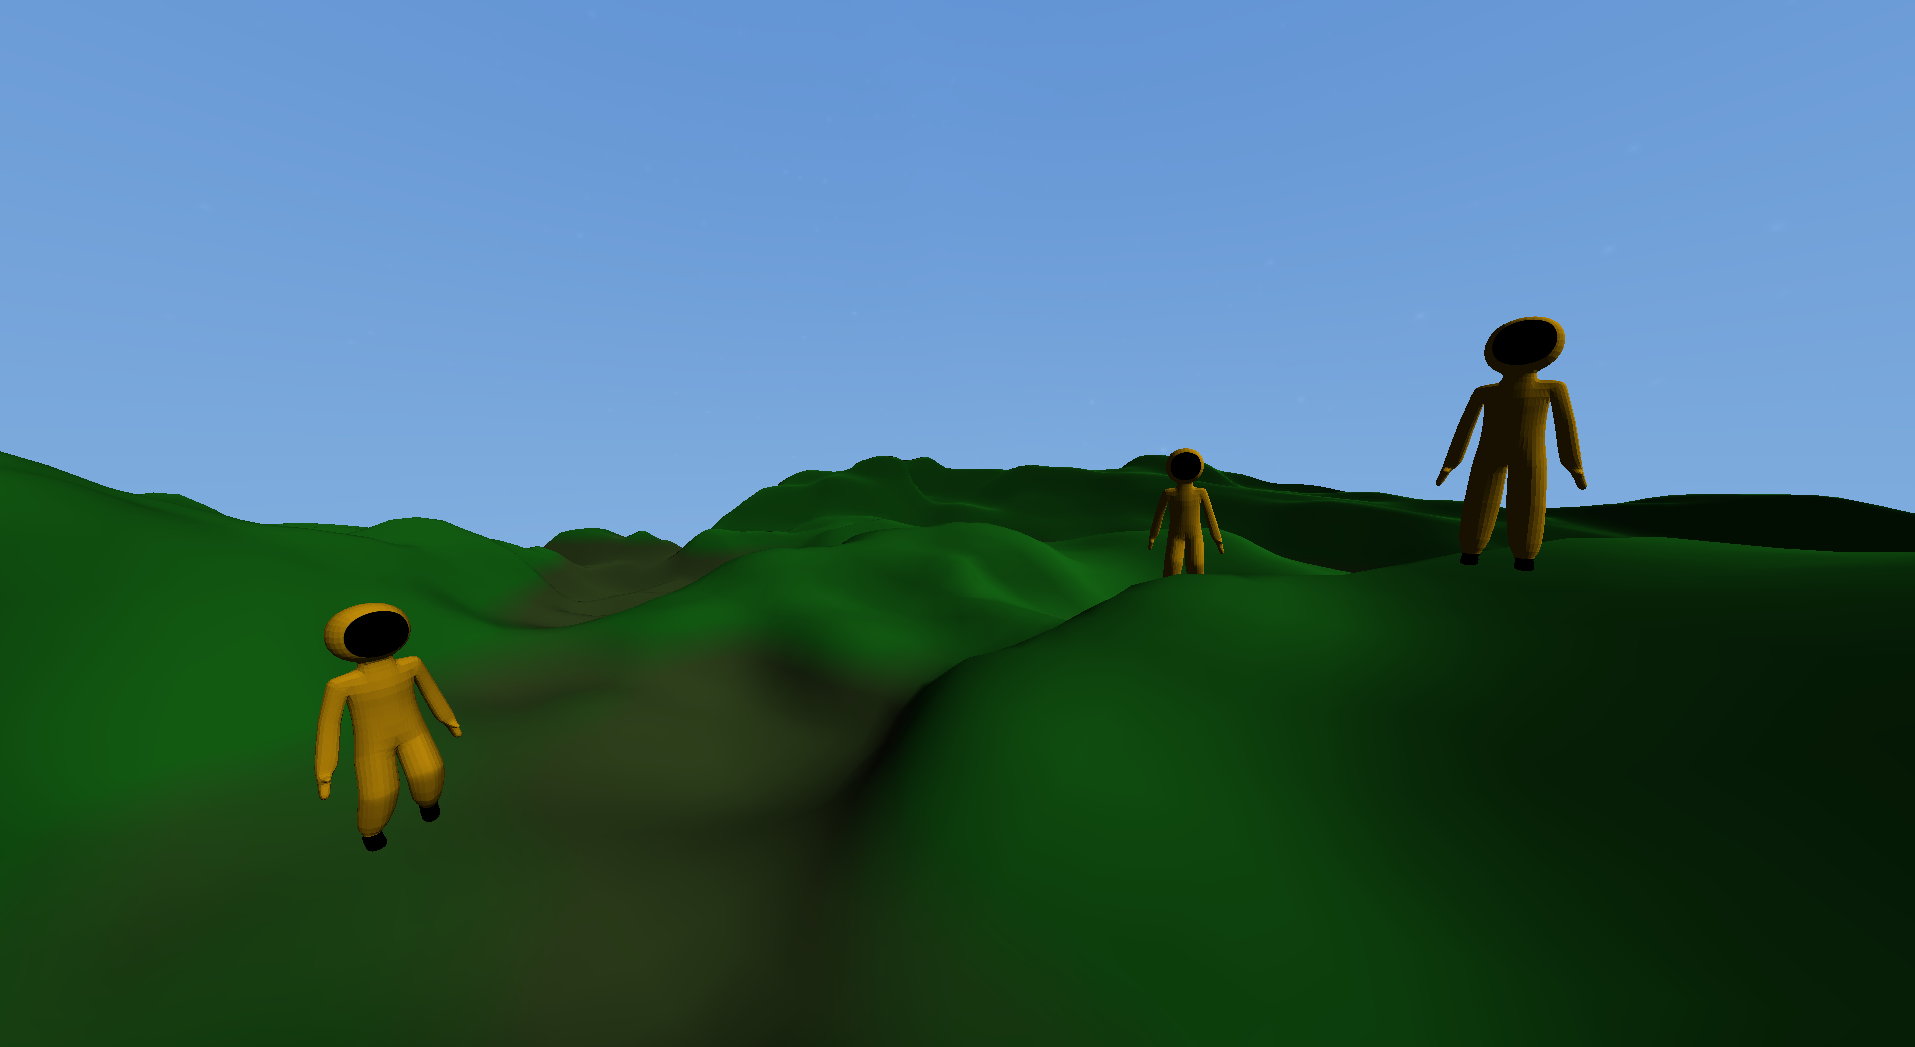
\includegraphics[width=0.8\textwidth]{chapters/problems/resources/hyperbolic-invisible.png}
    \caption{Hyperbolic geometry with the camera at the player's head.}
    \label{fig:hyperbolic_invisible}
\end{figure}

To make the scene appear visibly curved, the camera position was changed to a point with a relatively high value of the $y$ coordinate.
This solution, however, created a new problem, as the new camera's position made the gameplay look unnatural, as can be seen in \autoref{fig:hyperbolic_high_camera}.

\begin{figure}[!htb]
    \centering
    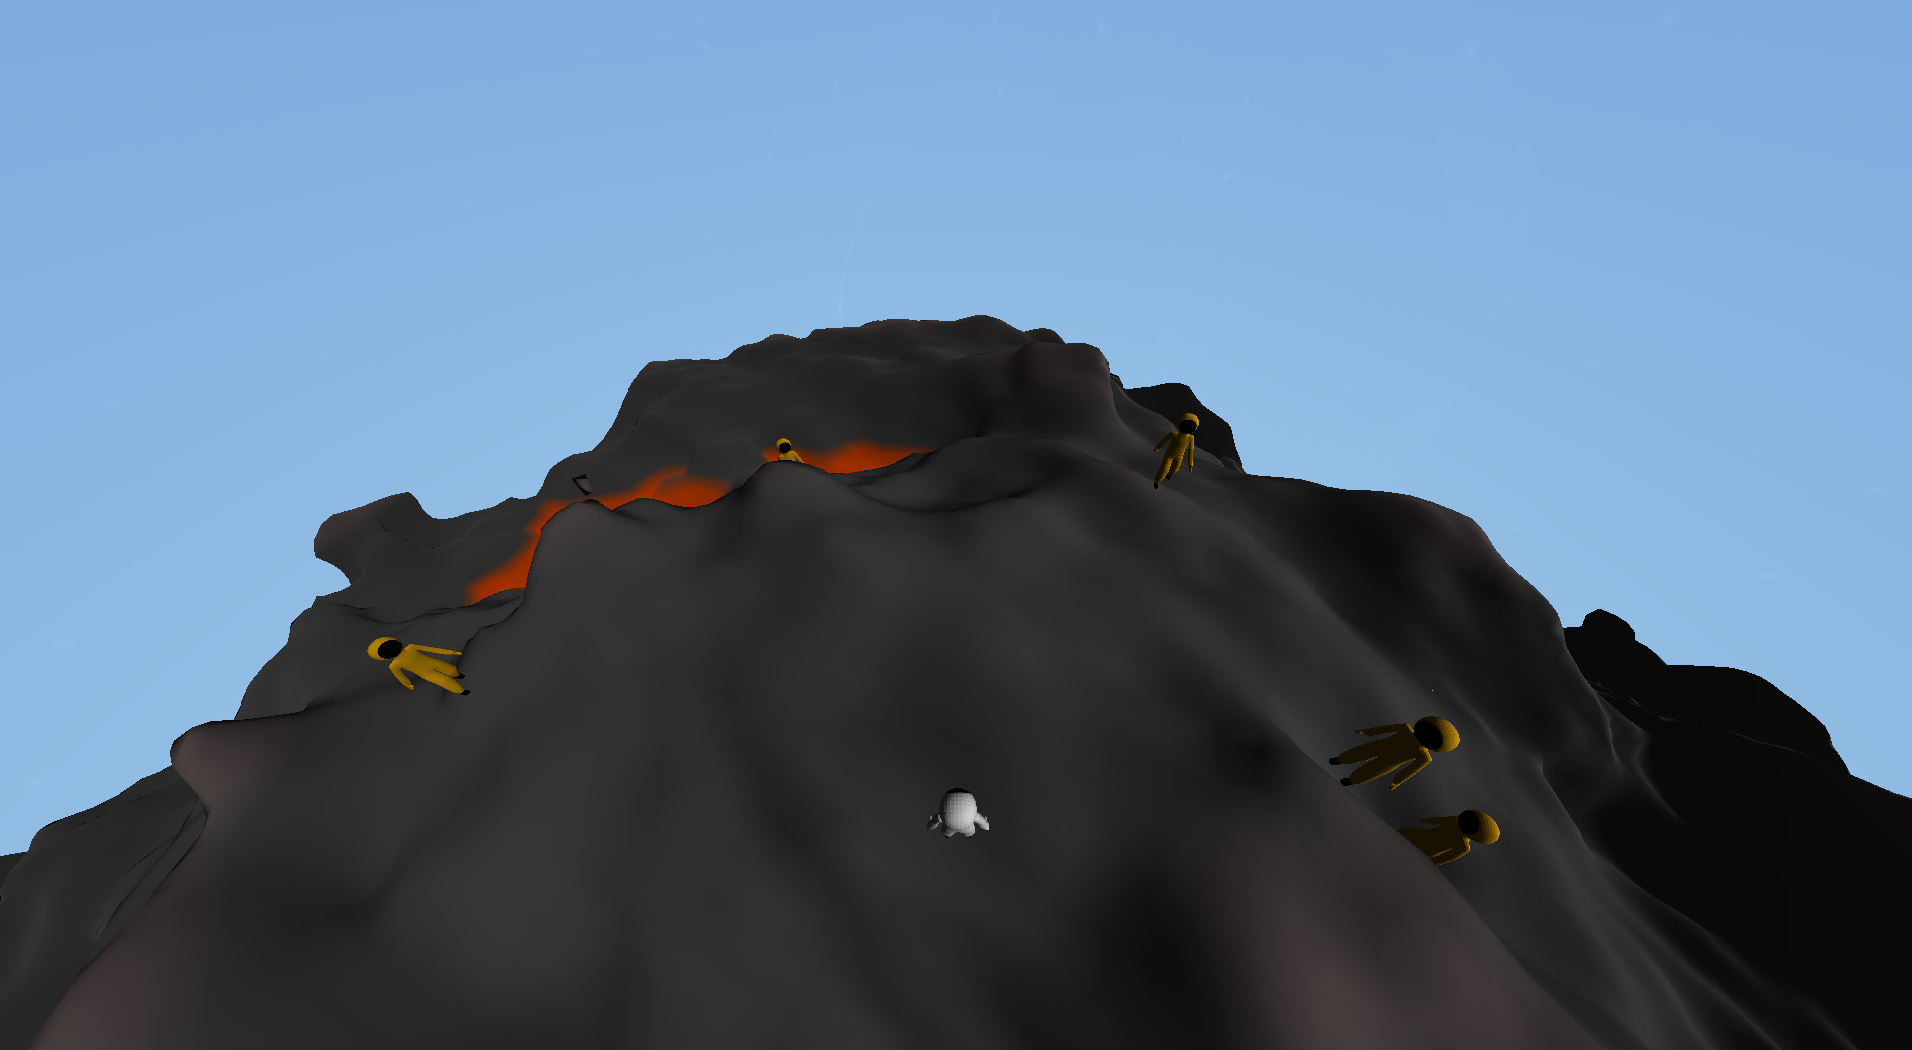
\includegraphics[width=0.8\textwidth]{chapters/problems/resources/hyperbolic-high-camera.png}
    \caption{Hyperbolic camera placed high above the player.}
    \label{fig:hyperbolic_high_camera}
\end{figure}

The solution to this problem was to move the whole world up.
The whole logic is as follows:
\begin{enumerate}
    \item The player inputs a key combination that moves him.
    \item The world is moved to simulate the effect of the player moving.
    \item The world is moved up to adjust for the raised camera.
    \item The frame is rendered.
\end{enumerate}

It is worth noting that "moving the world" only involves passing an appropriate vector to the shader.
The locations of the objects themselves are obviously not changed for performance reasons.